\section{The engineer chapter: distributions, failure modes, and controls}

\subsection{Scaling laws are resource-balance laws}

A standard empirical scaling model decomposes the test loss into terms associated with limited data and limited model capacity:
\[
E(T,d) \approx \left(\frac{T_c}{T}\right)^a + \left(\frac{d_c}{d}\right)^b.
\]
The equation should be read like a bottleneck model. Increasing $d$ cannot compensate indefinitely for inadequate $T$, and increasing $T$ cannot compensate indefinitely for inadequate $d$. For engineering, the important point is not the exact exponent but the structure: every improvement programme eventually becomes limited by the resource that is no longer growing appropriately \citep{kaplan2020scaling,hoffmann2022chinchilla}.

Synthetic data changes this picture because it changes what $T$ means. Ten million examples generated by the same teacher are not equivalent to ten million independent observations. We therefore distinguish:
\[
T_{\mathrm{raw}} \neq T_{\mathrm{effective}}.
\]
A useful conceptual decomposition is
\[
T_{\mathrm{effective}}
= T_{\mathrm{raw}}
\times q_{\mathrm{quality}}
\times q_{\mathrm{diversity}}
\times q_{\mathrm{independence}}
\times q_{\mathrm{freshness}}
\times q_{\mathrm{verification}}.
\]
This is not a universal statistical estimator. It is an engineering reminder that volume must be discounted when examples are correlated, stale, weakly verified, or narrow in support.

\subsection{Emergence: transition, threshold, or metric artefact?}

The literature on emergent abilities reports tasks that remain near random performance for smaller models and then improve sharply at larger scale \citep{wei2022emergent}. Engineers should separate three mechanisms:

\begin{enumerate}[leftmargin=*]
  \item \textbf{Internal transition.} The model discovers a reusable representation or composition.
  \item \textbf{Exposure threshold.} Rare but necessary examples finally become numerous enough.
  \item \textbf{Metric threshold.} A continuous internal improvement is converted into a discontinuous score such as exact match \citep{schaeffer2023mirage}.
\end{enumerate}

A system claim should therefore include both final metrics and continuous precursors: loss, margin, calibration, edit distance, residual reduction, partial correctness, and causal contribution of components.

\subsection{Zipf distributions and the long tail}

A ranked frequency distribution often follows
\[
p(i) = C i^{-\beta}, \qquad \beta>1.
\]
A small number of events dominate the mass, while many events are individually rare. In language, these can be rare words or constructions. In software engineering, they can be unusual dependency combinations, specific deployment states, rare load spikes, or uncommon failure sequences.

Uniform input sampling does not imply uniform output sampling. In the GCD example, uniformly sampled integer pairs induce approximately
\[
\Prob(\gcd(a,b)=k) \propto k^{-2}.
\]
Consequently, a model sees many examples with small GCDs and very few with large or structurally rare GCDs. Training distributions determine which arithmetic skills are learned and when \citep{charton2024gcd}.

\subsection{Perplexity is model-relative surprise}

For a token sequence $X=(x_1,\ldots,x_L)$, perplexity is
\[
\mathrm{PPL}(X)
= \exp\left(
-\frac{1}{L}\sum_{t=1}^{L}
\log p_\theta(x_t\mid x_{<t})
\right).
\]
Low perplexity indicates that the model assigned high probability to the observed continuation. High perplexity indicates surprise. It does not directly distinguish:

\begin{itemize}[leftmargin=*]
  \item useful novelty;
  \item domain-specific content;
  \item corrupted text;
  \item tokenization artefacts;
  \item missing context;
  \item genuine complexity.
\end{itemize}

Therefore, perplexity is a useful triage signal, not a quality certificate. It should be combined with data quality, semantic validity, novelty, and task relevance.

\subsection{The Hutter memory baseline}

The infinite-memory model intentionally removes generalization. Each input $i$ has a deterministic correct label $j_i$. The learner answers correctly only if the pair has appeared in the training set:
\[
\widehat f(i)=
\begin{cases}
 j_i, & \text{if }(i,j_i)\in D_T,\\
 \perp, & \text{otherwise.}
\end{cases}
\]
The test error is the probability mass of unseen events:
\[
E_T = \sum_{i\ge 1}p(i)(1-p(i))^T.
\]
For $p(i)\propto i^{-\beta}$,
\[
E_T \asymp T^{-(1-1/\beta)}.
\]
This is a scaling law produced by memorization and a heavy-tailed distribution \citep{hutter2021learning}. It is an essential baseline because it prevents a misleading interpretation:

\begin{keyidea}
A power-law improvement curve is evidence of increasing coverage. It is not, by itself, evidence of abstraction, reasoning, compositionality, or self-organization.
\end{keyidea}

For MMALS, the corresponding baseline is an exact context-to-route memory. Any claimed geometric or collaborative intelligence must outperform this baseline on unseen variants and novel compositions.

\subsection{Three ways to damage a tail}

\paragraph{Top-$p$ truncation.} Nucleus sampling keeps the smallest set of outcomes whose cumulative probability exceeds $p_0$. Everything outside the set receives probability zero. A small discarded probability mass can contain a very large number of rare possibilities.

\paragraph{Temperature narrowing.} If
\[
q_i^{(\tau)} \propto p_i^{1/\tau},
\]
then for a power law $p_i\propto i^{-\beta}$,
\[
q_i^{(\tau)} \propto i^{-\beta/\tau}.
\]
For $\tau<1$, the exponent increases and rare events become even rarer.

\paragraph{Finite sampling.} An event with probability $p_i$ is absent from a sample of size $N$ with probability
\[
(1-p_i)^N \approx e^{-Np_i}.
\]
Even a perfectly calibrated generator loses sufficiently rare events in a finite synthetic corpus.

These mechanisms differ operationally, but all reduce the coverage available to the next learner.

\subsection{Cut tails create a hard error floor}

If synthetic data omit all ranks above $k$, the modified Hutter scaling law is
\[
E_{\mathrm{test}}
\asymp T^{-(\beta-1)/\beta}
+ k^{-(\beta-1)}.
\]
The first term is ordinary finite-data error. The second is the missing probability mass beyond the cutoff. The second term does not decrease with $T$ \citep{dohmatob2024tails}.

\begin{figure}[H]
\centering
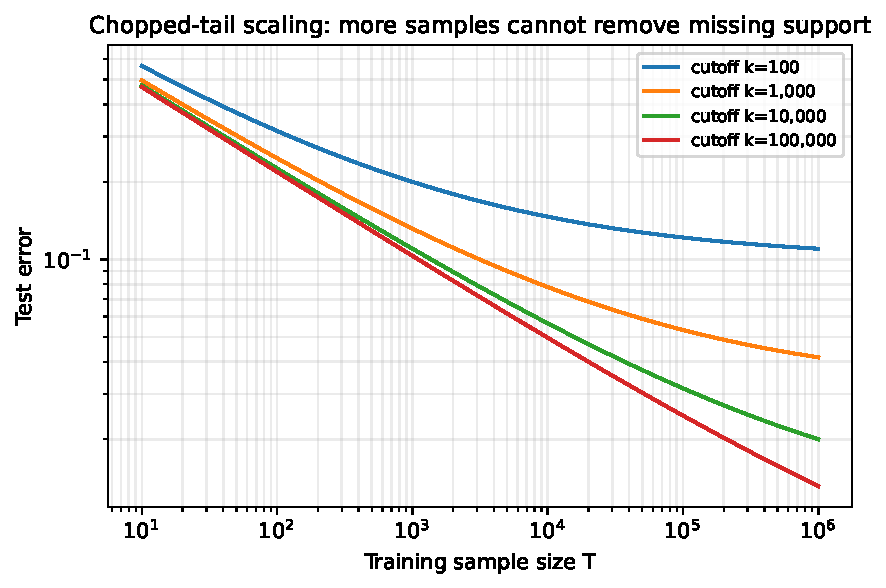
\includegraphics[width=0.86\textwidth]{figures/chopped_tail_scaling.pdf}
\caption{Original reconstruction of the chopped-tail scaling law. Each curve initially improves with sample size and then approaches a cutoff-dependent floor.}
\label{fig:chopped}
\end{figure}

The crossover occurs near
\[
T^\star \asymp k^\beta.
\]
Before $T^\star$, more samples help. After $T^\star$, the system is support-limited. The engineering action must change from ``generate more'' to ``restore missing regimes.''

\subsection{Recursive relabeling: same inputs, drifting truth}

Tail loss is not the only failure mode. The input distribution can remain unchanged while the labels become synthetic. In linear form,
\[
x\sim\mathcal N(0,\Sigma),\qquad
 y=x^\top w_0+\epsilon.
\]
A first ridge model estimates $\widehat w_1$, generates new labels, and a second model estimates $\widehat w_2$. The chain is
\[
P_{\Sigma,w_0,\sigma_0^2}
\rightarrow P_{\Sigma,\widehat w_1,\sigma_1^2}
\rightarrow P_{\Sigma,\widehat w_2,\sigma_2^2}
\rightarrow \cdots.
\]
Each generation can inherit previous bias and add new variance. More examples allow a student to fit the synthetic teacher more accurately, but do not automatically recover $w_0$ \citep{dohmatob2024regression}.

\begin{figure}[H]
\centering
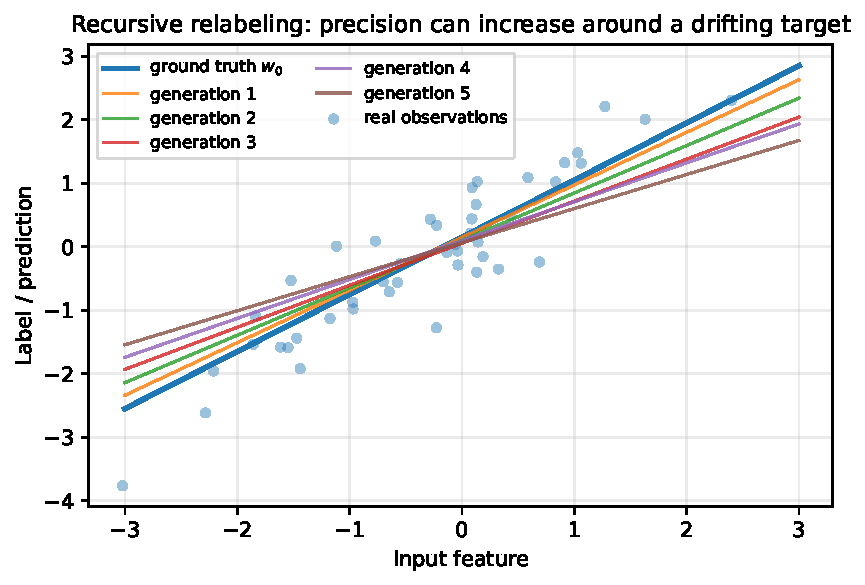
\includegraphics[width=0.82\textwidth]{figures/recursive_relabeling.pdf}
\caption{Conceptual recursive relabeling. Later generations may become precise around a drifting target.}
\label{fig:recursive}
\end{figure}

The practical analogy is instrument calibration. Repeatedly calibrating instrument $g+1$ against instrument $g$, rather than against the physical reference, can create a stable but biased chain.

\subsection{Model collapse is conditional, not mystical}

The broad literature shows different outcomes because the protocols differ. Collapse is more likely when:

\begin{itemize}[leftmargin=*]
  \item each generation replaces the original data;
  \item pseudo-label errors are treated as ground truth;
  \item sampling removes tails;
  \item model approximation errors are correlated across generations;
  \item the next learner has no independent corrective signal.
\end{itemize}

Stability is more plausible when:

\begin{itemize}[leftmargin=*]
  \item real data are retained or accumulated;
  \item fresh real observations continue to arrive;
  \item generated candidates are independently verified;
  \item the synthetic source targets under-covered regimes rather than only common ones;
  \item the mixture and regularization are adapted to lineage and uncertainty.
\end{itemize}

This reconciles apparently conflicting results such as recursive degradation \citep{shumailov2024curse,alemohammad2024mad} and stability under accumulation or controlled mixing \citep{bertrand2024stability,gerstgrasser2024inevitable}.

\subsection{When synthetic data help}

Let
\[
T=T_{\Real}+T_{\AI}.
\]
When real data are scarce relative to the preserved support, synthetic data can reduce finite-sample error:
\[
E_{\mathrm{test}}
\asymp (T_{\Real}+T_{\AI})^{-(1-1/\beta)}
+ k^{-(\beta-1)}.
\]
They densify the known support. They do not automatically extend it.

\begin{figure}[H]
\centering
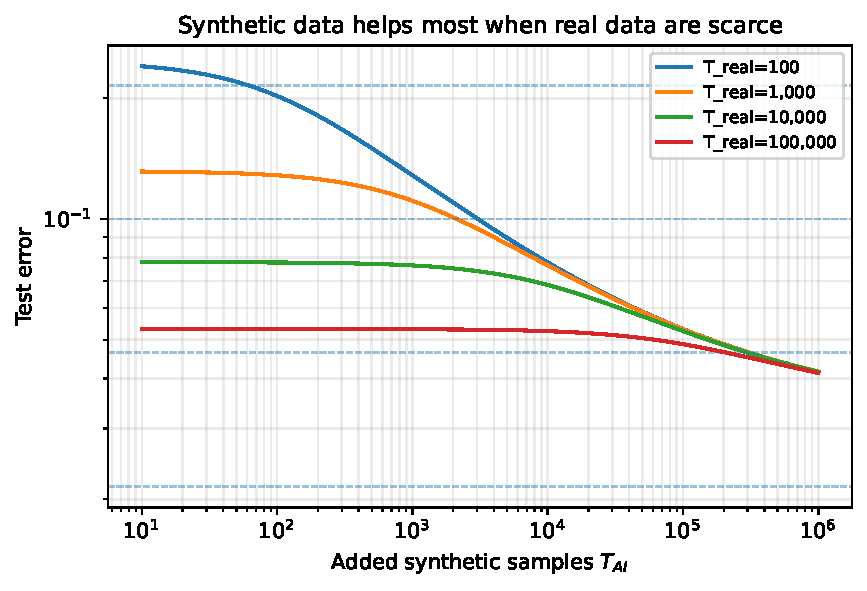
\includegraphics[width=0.86\textwidth]{figures/real_synthetic_mix.pdf}
\caption{Synthetic samples are most useful when the real sample is small. Benefits saturate at a support-dependent floor.}
\label{fig:mix}
\end{figure}

This creates four distinct business cases:

\begin{longtable}{p{0.20\textwidth}p{0.35\textwidth}p{0.35\textwidth}}
\toprule
\textbf{Use} & \textbf{Potential value} & \textbf{Main risk} \\
\midrule
Augmentation & More variation around known cases & Repetition disguised as diversity \\
Distillation & Transfer from a stronger model & Student inherits teacher's support ceiling \\
Rare-event generation & Increased exposure to selected regimes & Invalid or unrepresentative scenarios \\
Recursive self-training & Low-cost scale & Error and tail accumulation \\
\bottomrule
\end{longtable}

\subsection{Verification changes the economics}

The most constructive result is that an imperfect generator can be useful if good candidates can be recognized more cheaply than they can be generated directly \citep{feng2025verification}. The pipeline is:
\[
\text{seed data}
\rightarrow \text{generator}
\rightarrow \text{many candidates}
\rightarrow \text{verifier}
\rightarrow \text{filtered retraining set}.
\]

\begin{figure}[H]
\centering
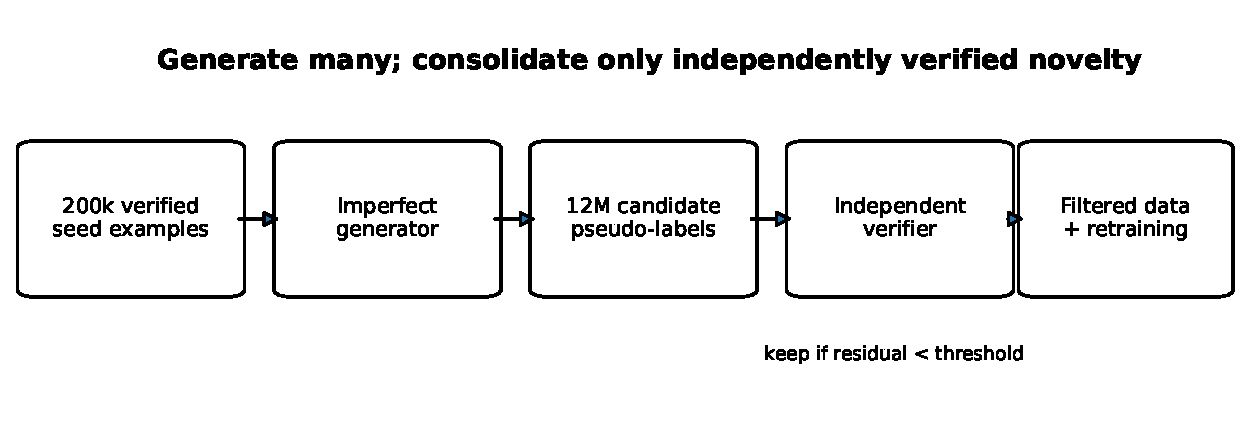
\includegraphics[width=0.96\textwidth]{figures/verification_bootstrap.pdf}
\caption{Verifier-based synthetic-data bootstrapping.}
\label{fig:verification}
\end{figure}

Let
\[
\phi = \Prob(\text{kept}\mid\text{correct}),\qquad
\psi = \Prob(\text{kept}\mid\text{incorrect}).
\]
A useful verifier has high $\phi$ and low $\psi$. Perfection is unnecessary; enrichment is necessary. The resulting system must still account for verification bias: a verifier that accepts only easy or conventional cases can create a new tail problem.

\subsection{Engineer checklist}

Before using synthetic data for training or testing, ask:

\begin{enumerate}[leftmargin=*]
  \item What independent information does the generator add?
  \item Which parts of the target distribution are absent or underrepresented?
  \item What are the sampling parameters and generation depth?
  \item Who or what provides the oracle?
  \item Is verification cheaper than direct production of correct labels?
  \item Are real anchors preserved and refreshed?
  \item Is success measured on a real, independent, uncontaminated evaluation set?
  \item Are average performance and rare-regime performance both reported?
  \item Can the system detect that more data no longer reduce the relevant uncertainty?
\end{enumerate}
